\chapter{Cross-Domain Synthesis, Parity Gates, and the Universality Claim}
\label{ch:cross-domain-synthesis}

ORIUS is written here as one universal argument, not as a witness-row result with
portability appendices.  The unifying object is the degraded-observation hazard: a
controller acts on an observed state, but safety belongs to the true state.  The
universal claim is therefore architectural and semantic from the start.  Every domain
chapter is asked the same question: can the ORIUS runtime detect degraded observation,
widen the observation-consistent state set, repair the candidate action, emit a
certificate, and document the exact non-claims for that domain?

\section{What the universal claim means}
The point of the manuscript is not to celebrate one plant.  The point is to show that
battery, vehicles, industrial plants, healthcare monitoring, navigation, and
aerospace can all be expressed through one safety-layer grammar: degraded observation,
reliability-aware inflation, action repair, bounded fallback, and auditable
certificates.  The claim is strong precisely because it is not a claim of shared
nominal control law, shared dynamics, or shared optimization objective.  It is a claim
about the runtime safety layer that sits between nominal intelligence and actuation.

\section{Equal-domain parity gate}
Universal framing does not remove evidence discipline.  The manuscript therefore uses
one explicit parity gate rather than many drifting summaries.  A domain only earns the
strongest universal rhetoric that matches its closure row: adapter correctness, data
and training surface, replay, soundness, fallback, CertOS lifecycle support, and
optional multi-agent portability all have to clear the same governed matrix.

\begin{table}[htbp]
\centering
\scriptsize
\caption{Equal-domain parity gate for the universal-first ORIUS book.}
\label{tab:orius-equal-domain-parity}
\resizebox{\textwidth}{!}{%
\begin{tabular}{p{2.5cm}ccccccccp{3.5cm}}
\toprule
\textbf{Domain} & \textbf{Adapter} & \textbf{Raw/Data} & \textbf{Train} & \textbf{Replay} & \textbf{Soundness} & \textbf{Fallback} & \textbf{CertOS} & \textbf{P5} & \textbf{Tier / Exact blocker}\\
\midrule
Battery Energy Storage & pass & locked\_reference & pass & pass & reference\_witness & safe\_hold\_validated & evaluated & evaluated & reference; battery\_reference\_row\\
Autonomous Vehicles & pass & verified & pass & pass & pass\_under\_ttc\_entry\_barrier\_contract & bounded\_brake\_fallback\_validated & evaluated & gated\_pending\_shared\_constraint\_surface & proof\_validated; multi\_lane\_and\_higher\_dimensional\_repair\_open\\
Industrial Process Control & pass & verified & pass & pass & pass & bounded\_runtime\_pass & evaluated & evaluated & proof\_validated; bounded\_to\_current\_plant\_family\\
Medical and Healthcare Monitoring & pass & verified & pass & pass & pass & bounded\_runtime\_pass & evaluated & gated\_pending\_shared\_constraint\_surface & proof\_validated; bounded\_to\_current\_monitoring\_and\_intervention\_contract\\
Navigation and Guidance & pass & blocked\_real\_data\_gap & blocked\_real\_data\_gap & portability\_only & blocked\_real\_data\_gap & bounded\_runtime\_pass & gated & gated & shadow\_synthetic; navigation\_real\_data\_row\_missing\\
Aerospace Control & pass & placeholder\_surface & placeholder\_surface & experimental\_replay\_only & experimental\_placeholder & bounded\_runtime\_pass & gated & gated & experimental; real\_multi\_flight\_safety\_task\_missing\\
\bottomrule
\end{tabular}}
\end{table}


\section{Current parity state}
The current manuscript clears four defended rows under one safety-layer vocabulary: battery as the deepest witness row, autonomous vehicles under the bounded TTC entry-barrier contract, industrial process control, and healthcare monitoring. Navigation remains gated by the missing defended real-data closure row. Aerospace remains gated by the absence of a real multi-flight runtime surface with stronger post-repair gain. A separate bounded public-flight ADS-B lane deepens aerospace runtime evidence without changing that official gate.

\section{Publication-readiness tiers}
The submission-readiness table below makes that distinction formal without asking the reader to absorb internal program language first. The bounded flagship target can clear as long as the manuscript, runtime, and calibration surfaces are strong while open rows remain explicitly gated. Navigation is promoted only when a locked real-data train/validate/replay row exists and clears replay, soundness, fallback, and runtime gates. Aerospace is promoted only when provider-approved multi-flight telemetry closes the governed parity lane with material post-repair gain on the defended flight safety object. Architecture universality is preserved; equal-domain universality is claimed only after every domain clears the same evidence, calibration, runtime, and governance gates.

\begin{table*}[htbp]
\centering
\scriptsize
\caption{Cross-domain claim-readiness summary for ORIUS. The bounded thesis claim can be defended with explicit gated rows, whereas equal-domain closure remains blocked until the open rows close by artifact, replay, and runtime evidence rather than by prose.}
\label{tab:orius-submission-readiness}
\resizebox{\textwidth}{!}{%
\begin{tabular}{p{2.3cm}p{2.3cm}p{2.3cm}p{2.3cm}p{2.3cm}p{2.3cm}p{2.3cm}p{2.3cm}p{2.3cm}p{2.3cm}}
\toprule
\textbf{Target tier} & \textbf{Reviewer composite /10} & \textbf{Critical gaps} & \textbf{High gaps} & \textbf{Calibration completeness} & \textbf{Runtime and governance completeness} & \textbf{Parity alignment} & \textbf{Readiness /100} & \textbf{Meets 93 gate} & \textbf{Verdict}\\
\midrule
bounded\_93\_candidate & 9.380 & 0 & 1 & 94.5 & 94.8 & 93.8 & 94.0 & True & achieved\_for\_bounded\_claim\_tier\\
public\_flight\_93\_candidate & 9.380 & 0 & 0 & 86.0 & 89.4 & 95.0 & 92.2 & True & achieved\_for\_bounded\_public\_flight\_support\_tier\\
equal\_domain\_93 & 8.060 & 2 & 1 & 75.7 & 82.0 & 83.3 & 80.5 & False & blocked\_pending\_equal\_domain\_parity\\
\bottomrule
\end{tabular}}
\end{table*}


\section{Canonical evidence versus supplemental diagnostics}
The evidence workflow used for this manuscript is intentionally two-lane.  The
canonical lane is the only lane allowed to change parity, score, and defended-domain
rhetoric.  The supplemental lane exists to hold bounded diagnostics, controlled
compute templates, and support experiments without allowing those artifacts to
impersonate official closure.  Supplemental or public-proxy evidence may deepen chapters but is non-authoritative for equal-domain promotion.

\begin{table*}[htbp]
\centering
\scriptsize
\caption{Two-lane ORIUS refresh discipline. Canonical results govern promotion; supplemental Hugging Face evidence is intentionally separated so support experiments cannot leak into the official parity surface.}
\label{tab:orius-refresh-lane-status}
\resizebox{\textwidth}{!}{%
\begin{tabular}{p{2.3cm}p{2.3cm}p{2.3cm}p{2.3cm}p{2.3cm}p{2.3cm}}
\toprule
\textbf{Lane} & \textbf{Source contract} & \textbf{Domains in scope} & \textbf{Latest status} & \textbf{Promotion allowed} & \textbf{Exact limit}\\
\midrule
official\_canonical\_results & canonical parity-closing raw sources and governed replay artifacts only & battery, av, industrial, healthcare, navigation, aerospace & navigation=blocked; aerospace=trainable\_plus\_public\_support & yes & The official parity matrix may only change when the canonical rows clear train, replay, soundness, fallback, and runtime checks under the existing gate.\\
supplemental\_hf\_results & small Hugging Face diagnostics and controlled compute templates & navigation and aerospace diagnostics; optional bounded support for other domains & supporting evidence only & no & Supplemental Hugging Face evidence cannot promote navigation or aerospace and cannot override the official parity gate.\\
aerospace\_public\_flight\_support & public ADS-B runtime support with explicit proxy-field provenance & aerospace chapter depth, runtime diagnostics, governance traces & bounded public-flight support built & no & This lane deepens aerospace evidence but cannot replace provider-approved multi-flight telemetry in the official parity gate.\\
\bottomrule
\end{tabular}}
\end{table*}


\begin{figure}[htbp]
\centering
\IfFileExists{reports/publication/fig_orius_equal_domain_parity_matrix.png}{%
\includegraphics[width=0.97\textwidth]{reports/publication/fig_orius_equal_domain_parity_matrix.png}%
}{%
\includegraphics[width=0.97\textwidth]{../reports/publication/fig_orius_equal_domain_parity_matrix.png}%
}
\caption{Shared defended-versus-gated view for the non-battery domain block. Chapters~40--44 refer back to this mini-matrix so the reader can see which rows are defended peers and which remain explicitly gated.}
\label{fig:ch40-44-shared-parity}
\end{figure}

\begin{figure}[htbp]
\centering
\IfFileExists{reports/publication/fig_orius_equal_domain_gate_timeline.png}{%
\includegraphics[width=0.92\textwidth]{reports/publication/fig_orius_equal_domain_gate_timeline.png}%
}{%
\includegraphics[width=0.92\textwidth]{../reports/publication/fig_orius_equal_domain_gate_timeline.png}%
}
\caption{Versioned equal-domain gate timeline written during the canonical closure refresh. The figure makes the operator procedure reader-visible instead of burying it in logs.}
\label{fig:orius-equal-domain-gate-timeline}
\end{figure}

\IfFileExists{paper/assets/tables/generated/tbl_ch40_44_cross_domain_support.tex}{%
\begin{table}[htbp]
\centering
\caption{Cross-domain support register for the active three-domain program.}
\label{tbl:ch40-44-cross-domain-support}
\begin{tabular}{lll}
\toprule
Domain & Role & Tier\\
\midrule
Battery Energy Storage & witness row & reference\\
Autonomous Vehicles & promoted row & runtime\_contract\_closed\\
Medical and Healthcare Monitoring & promoted row & runtime\_contract\_closed\\
\bottomrule
\end{tabular}
\end{table}
%
}{%
\begin{table}[htbp]
\centering
\caption{Cross-domain support register for the active three-domain program.}
\label{tbl:ch40-44-cross-domain-support}
\begin{tabular}{lll}
\toprule
Domain & Role & Tier\\
\midrule
Battery Energy Storage & witness row & reference\\
Autonomous Vehicles & promoted row & runtime\_contract\_closed\\
Medical and Healthcare Monitoring & promoted row & runtime\_contract\_closed\\
\bottomrule
\end{tabular}
\end{table}
%
}

\section{Evidence gaps and theory discipline}
The monograph is strongest when it states the asymmetry plainly: the runtime contract and theorem bridge travel farther than the current defended evidence. That is why the current edition distinguishes architectural universality from equal-domain closure. Where the theory surface is broader than the replay and
artifact surface, the claim is written as a bounded semantic or contractual
statement rather than as a flat cross-domain validation claim.

The calibration story is part of that discipline.  The manuscript carries one
cross-domain calibration matrix that separates theorem-backed calibration,
empirical bounded calibration, and conservative widening rather than merging them
into one ambiguous uncertainty narrative.

\begin{table}[htbp]
\centering
\caption{Calibration diagnostics for the active Battery + AV + Healthcare program.}
\label{tbl:orius-calibration-diagnostics}
\begin{tabular}{llllll}
\toprule
Domain & Tier Scope & OQE Bucket Coverage & Width Regime & Formal Calibration & Exact Limit\\
\midrule
Battery Energy Storage & reference & low: PICP 0.938, width 4937.813 | mid: PICP 1.000, width 4277.755 | high: PICP 0.906, width 934.616 & reliability bucket widths are emitted in three\_domain\_grouped\_width.csv & bounded grouped calibration evidence only; no conditional-coverage claim promoted & bounded to the promoted runtime target surface for this domain\\
Autonomous Vehicles & proof\_validated\_bounded & low: PICP 0.994, width 6.906 | mid: PICP 0.997, width 5.343 | high: PICP 0.999, width 3.513 & reliability bucket widths are emitted in three\_domain\_grouped\_width.csv & bounded grouped calibration evidence only; no conditional-coverage claim promoted & bounded to the promoted runtime target surface for this domain\\
Medical and Healthcare Monitoring & proof\_validated\_bounded & low: PICP 0.845, width 0.952 | mid: PICP 0.834, width 1.381 | high: PICP 0.853, width 1.396 & reliability bucket widths are emitted in three\_domain\_grouped\_width.csv & bounded grouped calibration evidence only; no conditional-coverage claim promoted & bounded to the promoted runtime target surface for this domain\\
\bottomrule
\end{tabular}
\end{table}


\begin{figure}[htbp]
\centering
\IfFileExists{reports/publication/fig_orius_calibration_coverage_matrix.png}{%
\includegraphics[width=0.88\textwidth]{reports/publication/fig_orius_calibration_coverage_matrix.png}%
}{%
\includegraphics[width=0.88\textwidth]{../reports/publication/fig_orius_calibration_coverage_matrix.png}%
}
\caption{Cross-domain calibration coverage matrix by domain and slice family. The figure stays synchronized to the generated calibration diagnostics table.}
\label{fig:orius-calibration-coverage-matrix}
\end{figure}

\section{Why the gate stays reader-visible}
The parity gate is not an embarrassing appendix.  It is the mechanism that lets ORIUS
argue for a field-level runtime safety layer without pretending that every supported
domain is already equally mature.  The manuscript is strongest when
architecture-level universality and evidence-level parity are both explicit and both
governed.

\section{T9 universality impossibility boundary}
\label{sec:monograph-t9-universal-impossibility}
The current impossibility boundary is not a contradiction of the ORIUS architecture.
It is the point at which a domain remains structurally compatible with the runtime
contract but fails to close the relevant true-state violation event under the present
repair geometry or telemetry surface.

\section{T10 lower-bound interpretation}
\label{sec:monograph-t10-lower-bound}
The lower-bound interpretation in the monograph says that insufficient recoverable
information in the degraded observation channel limits what any runtime repair layer
can certify.  ORIUS can still govern fallback and logging there, but it cannot invent
theorem-grade closure from missing signal.

\paragraph{Universality completeness statement}
\label{par:monograph-universality-completeness}
ORIUS is complete as a universal architectural layer when every supported domain can
express degraded observation, admissible repair, and certificate semantics through one
runtime contract, while empirical promotion stays tied to the governed parity matrix
rather than assumed by analogy. Navigation is promoted only when a locked real-data train/validate/replay row exists and clears replay, soundness, fallback, and runtime gates. Aerospace is promoted only when provider-approved multi-flight telemetry closes the governed parity lane with material post-repair gain on the defended flight safety object. Architecture universality is preserved; equal-domain universality is claimed only after every domain clears the same evidence, calibration, runtime, and governance gates.
